\documentclass[./../../paper.tex]{subfiles}
\graphicspath{{\subfix{./../../figures/}}}

\begin{document}

\section{Determine the Evolutionary Algorithm Configurations}
As explained in \autoref{sec:evolutionary}, there are many possible configurations for an evolutionary algorithm. Therefore, we run simulations for all possible combinations of operators. We use the results, to filter out operators for subsequent evaluation steps that may not be promising.

\subsection{Experimental Setup}
\label{sec:exp1}
 To avoid confusion, we refer to each unique phase combination as a configuration. For instance, one configuration would consist of \attention{a DatabBasedInitiator, an ElitismSelector, a OnePointCrosser, SamplinBasedMutator and a FittestSurvivorRecombiner}. We refer to a specific configuration in terms of its abbreviated operators. For instance, the earlier example is denoted as \attention{DBI-ES-OPC-SBM-FSR}.

The configuration set contains \attention{144} elements. We choose to run each configuration for \attention{50} evolution cycles. For all configurations, we use the same set of \attention{5} factual \glspl{instance}, which are randomly sampled from the test set. We decide to return a maximum of \attention{1000} counterfactuals for each factual case. Within each evolutionary cycle, we generate \attention{100} new offsprings. We keep the mutation rate at \attention{0.1} for each mutation type. Hence, across all cases that are mutated, the algorithm inserts, deletes, and changes \attention{1\%} of events. 

% After retrieving the results, we fit a linear mixed-effects model to determine the importance of each configuration. Here, we use the resulting viability as a dependent variable and each phase as independent variable. We adjust the model according to their configuration, as we retrieve \attention{50} samples per configuration. If a phase-type strongly affects the dependent variable and the resulting change is deemed significant, we can draw conclusions about the full configuration. Furthermore, preliminary results showed that many of the configurations have a zero feasibility. Hence, we also incorporate the insights gained from using feasibility as a dependent variable.

\subsection{Results}

% TODO: Change plots to matplotlib plots
\begin{figure}[htbp]
    \centering
    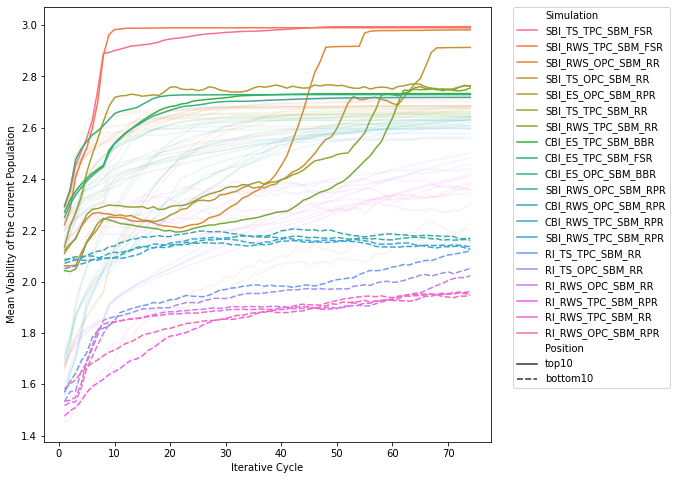
\includegraphics[width=\textwidth]{figures/generated/exp1_effect_on_viability_top10_last10.png}
    \caption{This figure shows the average viability of the \attention{10} best and worst configurations. The x-axis shows how the viability evolves for each evolutionary cycle.}
    \label{fig:average-viability}
\end{figure}

\noindent \autoref{fig:average-viability} shows the bottom and top-\attention{k} configurations based on the viability after the final iterative cycle. We also show how the viability evolves for each iteration.\attention{change evolutionary cycle to iterative cycle} The results reveal a couple of patterns. 
First, all of the top-\attention{k} algorithms use \attention{either CaseBasedInitiator or SampleBasedInitiator} as initiation operation. In contrast, the bottom-\attention{k} all use \attention{RandomInitiator} as initialisation. 
Second, we see that most of the top-\attention{k} algorithms use the \attention{ElitismSelector}. 

The complete table of results is in \autoref{tbl:average-viability}.
\needsattachment{tbl:average-viability}

% \noindent  shows for the \attention{average feasibility for each configuration}. It does not surprise, that the \attention{FactualInitiator} remains at a low feasibility as deviations will often lead to infeasible counterfactuals. The evolutionary algorithm remains at a local optimum without exploring other solutions. Furthermore, we see that most configurations reach at most \attention{0.04} feasibility, while the initialisation with the \attention{DataDistributionSample} initiator reaches higher values. 


\begin{figure}[htbp]
    \centering
    \begin{subfigure}[c]{0.9\textwidth}
        \centering
        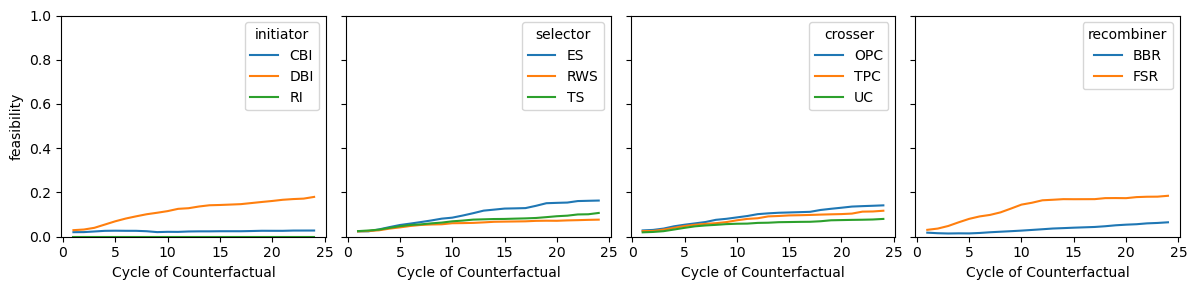
\includegraphics[width=\textwidth]{figures/generated/exp1_feasibility.png}
        \label{fig:exp1-feasibility}    
    \end{subfigure}
    \hfill
    \begin{subfigure}[c]{0.9\textwidth}
        \centering
        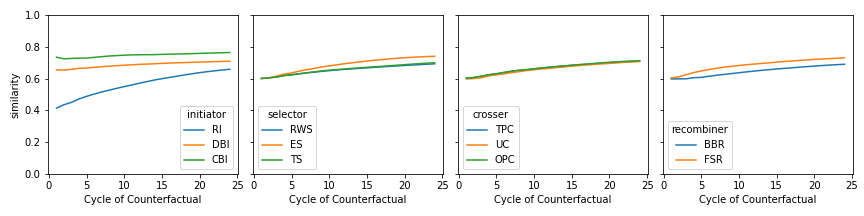
\includegraphics[width=\textwidth]{figures/generated/exp1_similarity.png}
        \label{fig:exp1-similarity}
    \end{subfigure}
    \hfill
    \begin{subfigure}[c]{0.9\textwidth}
        \centering
        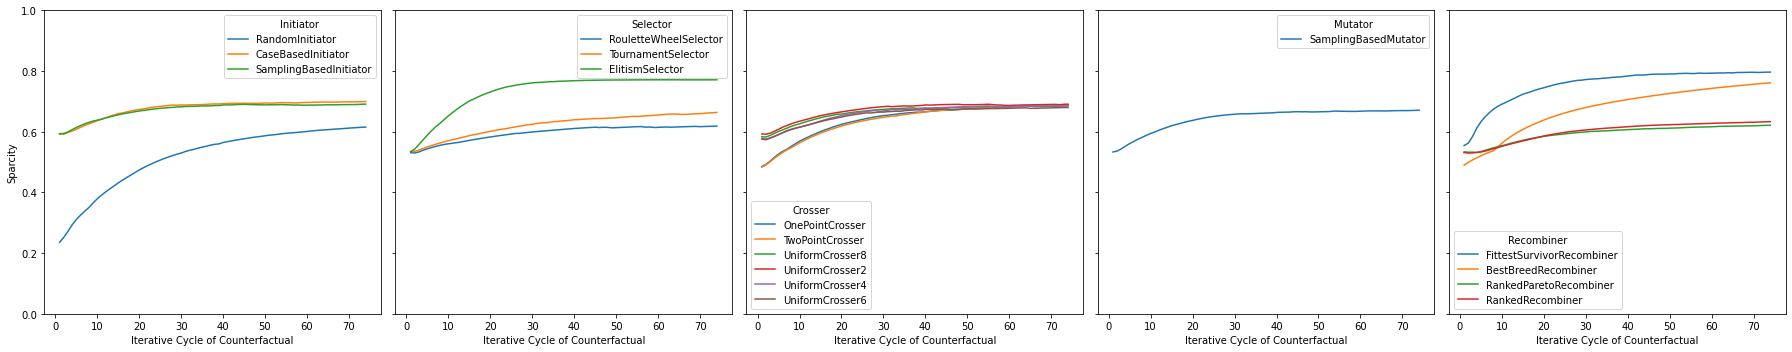
\includegraphics[width=\textwidth]{figures/generated/exp1_sparcity.png}
        \label{fig:exp1-sparcity}
    \end{subfigure}
    \hfill
    \begin{subfigure}[c]{0.9\textwidth}
        \centering
        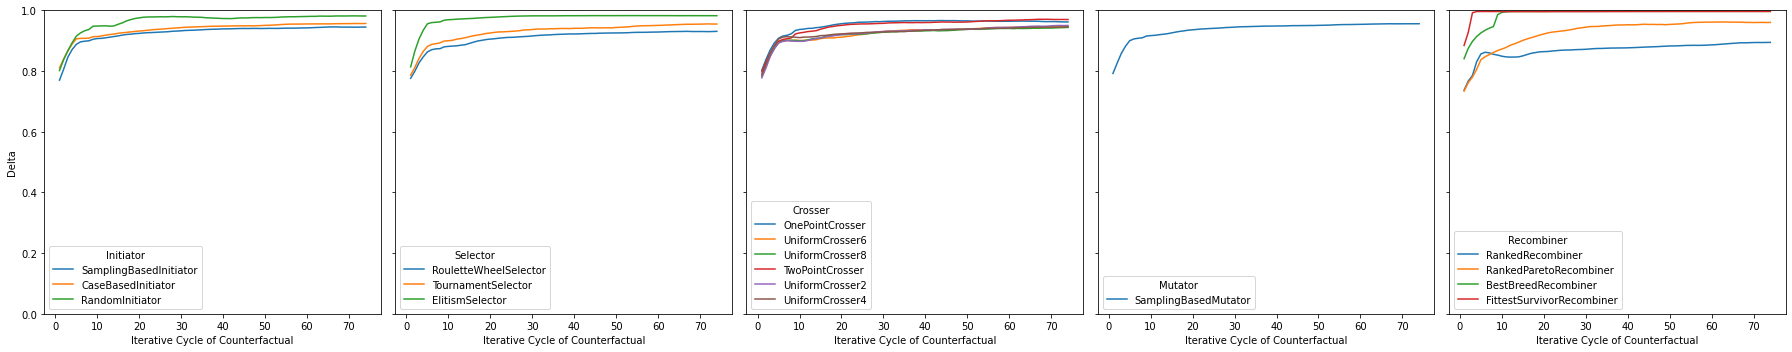
\includegraphics[width=\textwidth]{figures/generated/exp1_delta.png}
        \label{fig:exp1-delta}
    \end{subfigure}
    \caption{Shows the evolution of each viability measure over the entire span of iterative cycles. Each figure adjust the respective operator type by taking the average over all other operator types. \attention{Make sure, that the legends are aligned in color.}}
    \label{fig:exp1-measure}
    
\end{figure}

In \autoref{fig:exp1-measure}, we see the effects of each operator type, except the mutation operation. 

Starting with some commonalities accross operator-type and measure, the figure shows that the initiator heavily determines the starting point for each measure. For instance, the \attention{RandomInitiator} starts well below the other initiator operations when it comes to sparcity and similarity. 
Another noteworthy general observation is the delta measure\attention{Change some of the names to align with Dice4EL}. Here, for each operator type we see a movement towards the highest possible delta value. Hence, most configurations are capable of changing the source class to the desired class. 

In terms of viability \autoref{fig:exp1-feasibility}, shows an increase only for cases, in which the \attention{SampleBasedInitiator} is used. Similar holds for recombination with \attention{FittestSurvivorRecombiner}.

The results for the selection operator type are undeniably in favor of \attention{ElitismSelector} for all viability measures. The same holds for the recombination operation. Here, the \attention{FittestSurvivorRecombiner} yields better results.

When it comes to the crossing operation, the results indicate, the differences between \attention{OnePointCrosser} and \attention{TwoPointCrosser} are inconclusive for all viability measures except feasibility. One can explain that by noting, that both operations are very similar in nature. However, cutting the sequence only once retains produces less impossible sequences for the child sequences.



\subsection{Discussion}
% The reasons for the superiority of \attention{FactualInitiator} are clear.If we start the model with the factuals as initial population, the factual will already have a viability of at least 2 as similiarity and sparcity have to be at their maximal value. As the prediction model tends to only assign scores close to the extremes, the favorable change of an event attribute often yields a strong bias which is often correct. Hence, the viabilities often reach a viability of around 3. The only way to reach a higher viability for factually inititiated counterfactuals is to approach the pareto-surface by increasing the feasibility. In other words, one would have to increase feasibility without significantly decreasing the scores for similarity, sparcity and the improvement. Similarly, it is no surprise, that the \attention{FactualInitiator} has a negative effect on the feasibility, as it is difficult to find a case which is even more likely than a case that was directly sampled from the log.

Moving forward, we have to choose a set of configurations and also determine suitable hyperparameters for each. In the next experiment we consider the following configurations: We choose the \attention{SampleBasedInitiator} as it might increase our chances to generate feasible variables. 

For selection, we will use the \attention{ElitismSelector}, as it generally appears to return better results. 
% Furthermore, we include the \attention{FactualInitiator}, as it would be interesting whether we can reach better results, by changing parameters. For selection, we will use the \attention{ElitismSelector and RouletteWheelSelector}. The former because it seems to be consistently better than the other selectors. The latter because, we suspect that the negative effect is highly bised by the results of the \attention{FactualInitiator}. 

Furthermore, we choose to move forward with the \attention{OnePointCrosser}. This crossing operation is slightly better in yielding feasible results. 

For selection and recombination, we use the \attention{ElitismSelector} and the \attention{FittestIndividualRecombiner}, respectively. They all outcompete their alternatives for all similarity, sparcity and feasibility.

In the next experiment we vary mutation rates, using \attention{SBI-ES-OPC-SBM-FIR}.
% TODO: Use constants for the indivdual config names.
\end{document}